\section{Overview su cross platform mobile}
Al momento di scegliere come implementare l'applicazione mobile per CAMUS sono state considerate due opzioni: la creazione di un'applicazione nativa inizialmente solo per Android, per poi estendere la compatibilit� su iOS, oppure l'utilizzo di strumenti cross platform, funzionanti su pi� di un sistema operativo mobile.
Questa esigenza � nata dal fatto che il mercato delle app mobile sta crescendo in maniera esponenziale e le competenze richieste agli sviluppatori sono molto variegate per sviluppare applicazioni native.
Per esempio per quanto riguarda lo sviluppo iOS � necessario conoscere come linguaggi di programmazioni Objective-C e Swift, per Android ci si basa principalmente su Java e per Windows Phone � necessario utilizzare C-sharp \textcolor{red}{(Non mi prende il cancelletto)}, senza dimenticare altri sistemi operativi meno diffusi o emergenti (Tizen, Ubuntu Touch, ecc.).
Gli strumenti di sviluppo \textbf{cross-platform} solitamente si basano sul principio di \virgolette{write once run everywhere}, cio� il codice viene scritto una volta sola per creare applicazioni per diverse piattaforme, permettendo quindi di limitare le competenze richieste ai programmatori. 
\upe possibile identificare due famiglie di strumenti per la programmazione multi piattaforma:
\begin{enumerate}
	\item \textbf{Rendering tramite componenti nativi} In questa famiglia il rendering dell'applicazione viene fatto utilizzando le API grafiche native del sistema operativo di destinazione.
	\textcolor{red}{allungare + esempi}
	\item \textbf{Rendering tramite WebView} In questa famiglia il rendering dell'applicazione � svolto in una pagina web, che viene caricata delle volte in un container composto da componenti nativi.
	In questo caso � possibile programmare l'applicazione come se fosse una pagina web, implementandolo allo stesso modo di un sito web per browser.
	Purtroppo questo nel \virgolette{look and feel} dell'applicazione non � sempre un vantaggio, perch�, nonostante le possibilit� di scelta grafiche e di comportamento siano molteplici, le prestazioni possono risentire del fatto che si stia interagendo con una pagina web e non con una applicazione nativa.
\end{enumerate}

 


\section{Tecnologie utilizzate}
Per la creazione di CAMUS si � scelto di utilizzare anche lato backend degli strumenti che siano implementabili in maniera semplice e dove la suddivisione in moduli singoli riutilizzabili assuma un ruolo di primo piano. Per questo motivo si � scelto di utilizzare degli strumenti tecnologici che sono all'avanguardia nello svolgere questo compito, come React e la sua derivazione per la programmazione mobile React Native. Successivamente � introdotta la parte logica dell'applicazione con il funzionamento architetturale dell'aggiornamento dati, con il paradigma Flux.

\subsection{React}

React nasce come libreria open-source rilasciata nel 2013 da Facebook, che permette di ottimizzare le visualizzazioni delle pagine HTML, utilizzando componentine racchiudono altri specificati come HTML tag personalizzati.
Essa proviene da XHP, che � un framework HTML per il linguaggio PHP, ed � stata prima utilizzata nel newsfeed di Facebook nel 2011 e pi� tardi in Instagram.com.
Le principali funzionalit� in React sono le seguenti:
\begin{itemize}
	\item \textbf{One-way data flow} Le propriet�, un set di valori immutabili, sono passati al componente figlio all'interno del suo tag HTML.Il componente figlio non pu� modificare direttamente nessuna propriet� che gli � stata passata, ma pu� passare funzioni che possono modificare il valore. \textcolor{red}{(introdurre esempio)}
	\item \textbf{Virtual DOM}
	React crea una propria struttura dati in memoria, che calcola le differenze risultanti e aggiorna il DOM HTML risultante nella pagina in modo efficiente. In questo modo il programmatore pu� scrivere codice come se l'intera pagina � ricaricata ogni volta, mentre � la libreria React a stabilire quali siano i componenti che vadano sostituiti e quali no. 
	\item \textbf{JSX}
	I componenti React sono solitamente scritti in JSX, un'estensione JavaScript che permette di quotare facilmente HTML e utilizzarne la sintassi per i tag per renderizzare i sottocomponenti
\end{itemize}

\subsection{React Native}
React Native � una libreria open-source rilasciata nel 2015 sempre da Facebook, proponendosi come estensione del framework React per quanto riguarda le applicazioni mobile.
Le principali differenze con React sono dovute alla difficolt� maggiore di sviluppare un framework per le applicazioni mobile. 
Quando si sviluppa sul web, semplicemente si salvano i file modificati e si ricarica la pagina, cosa che non � possibile fare con le applicazioni mobile, perch� � necessaria una nuova compilazione per vedere i cambiamenti apportati.
Con React Native � possibile migliorare l'esperienza d'uso sulle piattaforme mobile rispetto al web. Come primo aspetto si pu� accedere ai componenti specifici dell'interfaccia utente, come le mappe, i picker e gli switch, anche se tuttavia possono essere reimplementati e modificati.

\textcolor{red}{Aggiungere grafico e spiegazione architettura react native}

Lo sviluppo con React Native si basa sull'utilizzo di un server locale in \emph{node.js} che permette il caricamento delle modifiche dell'applicazione sul dispositivo senza ricompilare l'applicazione. Questo server, il quale ha la funzione di packager, invia un bundle contente tutti i file JavaScript necessari per far funzionare l'applicazione. Questo funziona fino a quando le modifiche sono relative esclusivamente alla parte di codice JavaScript, mentre per quanto riguarda le modifiche a livello di codice nativo � sempre necessaria una nuova compilazione. Per esempio, quando � stato il momento di installare alcune librerie grafiche collegate ad elementi nativi � stato necessario apportare modifiche anche ai file di configurazione dei progetti Android e iOS, dato che diventavano necessari anche file aggiuntivi alla compilazione.

\textcolor{red}{Da Completare meglio}

\subsection{Flux}

Flux � il pattern architetturale per gestire il flusso dei dati all'interno dell'applicazione. \upe complementare alla gestione delle view di React, in cui i componenti sfruttano un flusso di dati unidirezionale, come espresso in Figura \ref{fig:flux}.

\begin{figure}[ht]
	\centering
	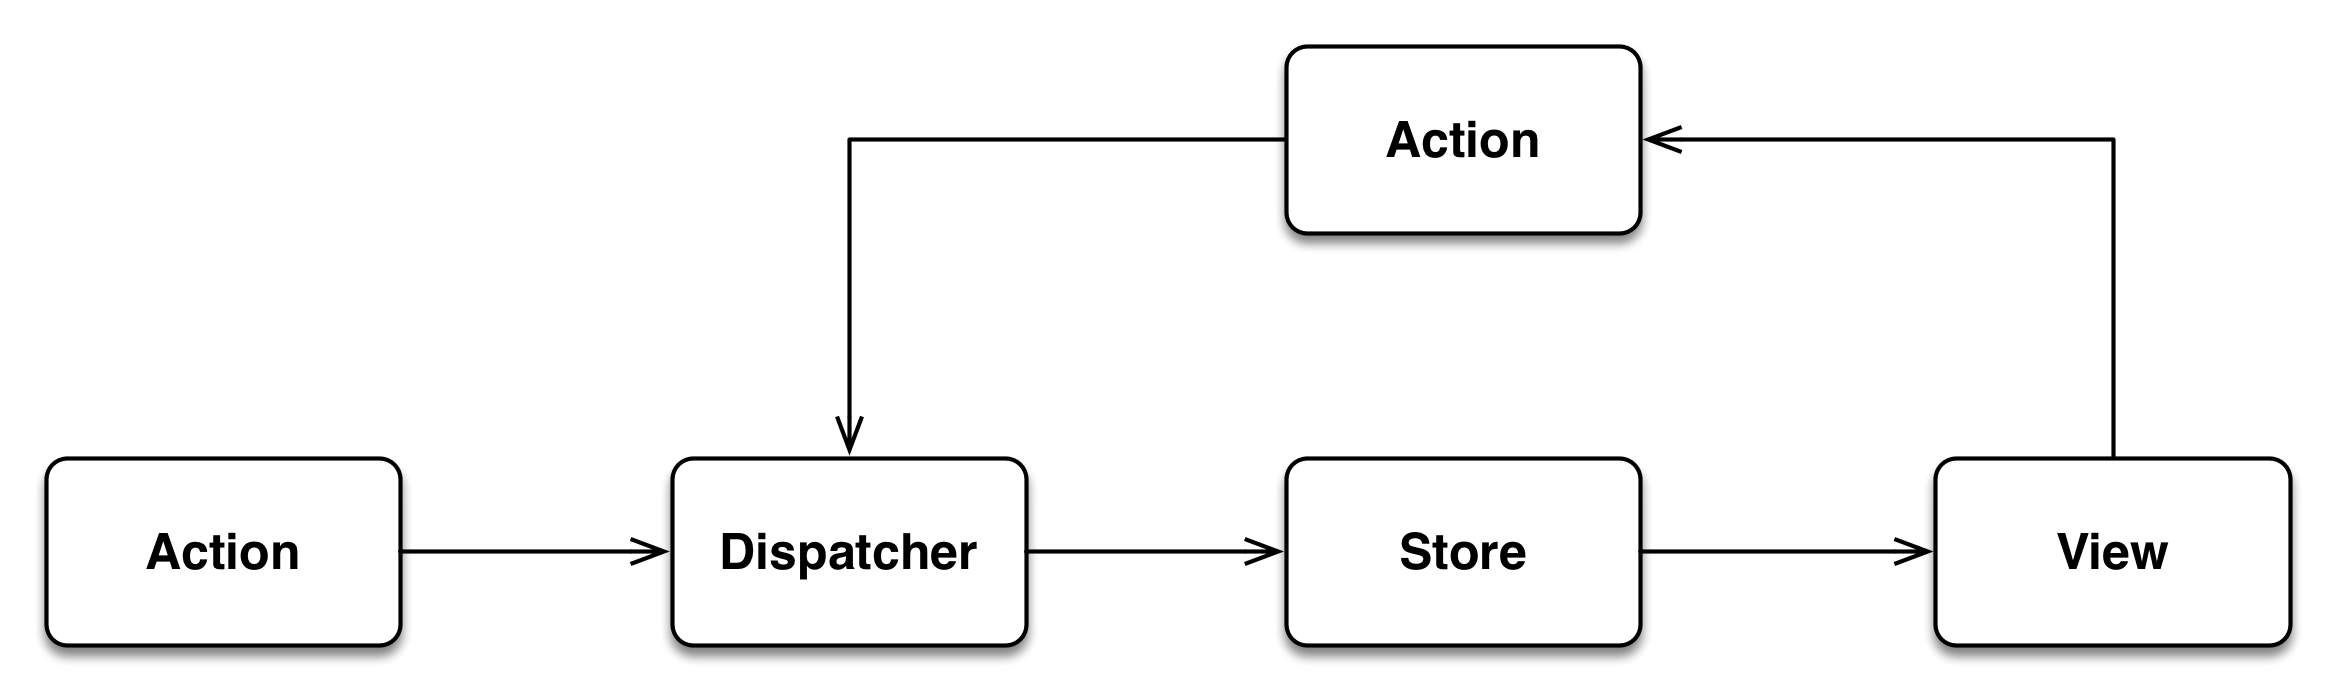
\includegraphics[width=\textwidth]{6-implementazione-app/immagini/flux.png}
	\caption{Flusso dati unidirezionale Flux}\label{fig:flux}
\end{figure}
Si tratta fondamentalmente di una modifica del pattern MVC (Model View Controller), al quale vengono introdotte alcune migliorie.
Le applicazioni Flux, come si vede nella medesima figura, hanno quattro tipologie di componenti principali: 
\begin{enumerate}
	\item \textbf{Dispatcher}
	Il \emph{Dispatcher} � l'hub centrale che controlla tutto il flusso dei dati dell'applicazione. \upe essenzialmente un registro di callback alle \emph{Store} e possiede un meccanismo semplice per distribuire le \emph{Action} verso le \emph{Store}. Man mano che l'applicazione cresce di dimensioni, il \emph{Dispatcher} assume un'importanza sempre maggiore, perch� pu� essere sfruttato per gestire le dipendenze tra le \emph{Store} invocando le callback registrate in un ordine specifico, talvolta anche attendendo la conclusione dell'aggiornamento delle altre \emph{Store} 
	\item \textbf{Store}
	Le \emph{Store} contengono lo stato dell'applicazione e la logica, e il loro ruolo � molto simile al modello nel pattern MVC, ma in Flux hanno il compito di modellare lo stato per un particolare dominio all'interno dell'applicazione
	\item \textbf{View}
	L'implementazione delle view proposta da React si sposa perfettamente con quella necessaria per Flux. Si tratta di un misto tra la view e il controller in MVC, perch� permette al codice di ricevere i dati dalle store e passare questi dati direttamente ai discendenti per creare ogni singola sezione della pagina. Quando riceve un evento dalle \emph{store}, richiede i nuovi dati attraverso i \emph{getter} delle \emph{store}, per poi aggiornare il proprio stato interno e renderizzarlo a cascata utilizzando tutti i sottocomponenti.
	\item \textbf{Action} Con il termine \emph{Action} si intende il payload di dati che viene mandato al metodo esposto dal \emph{dispatcher}, il quale come espresso nella sua spiegazione, poi penser� a come inviare i dati alle \emph{store}.
\end{enumerate} 
\section{Struttura dei file di mashup}



\section{Rendering delle view}

abc

\section{Flusso di esecuzione}

abc

\section{Utilizzo dei dati}

abc

\subsection{Costruzione query GraphQL}

abc

\subsection{Gestione paginazione}

abc

\subsection{Gestione errori ed aggiornamenti}

abc

\section{Servizi di supporto}

abc